\clearpage
\VerdierPhysicalPageAnchor{0100}%
\begingroup
\small
\setlength{\abovedisplayskip}{3pt plus 2pt minus 2pt}%
\setlength{\belowdisplayskip}{3pt plus 2pt minus 2pt}%
\setlength{\jot}{2pt}%
\VerdierSemanticAnchor{ch1-3-3-5-proof-completion}
事实上，第一项断言是 (3.2.2) 的直接推论；由命题 (3.2.12)，存在态射
$c(I)\colon c(g)\longrightarrow c(c(D))$，使得下图

\VerdierSemanticAnchor{ch1-3-3-5-isomorphism-diagram}
\begin{center}
  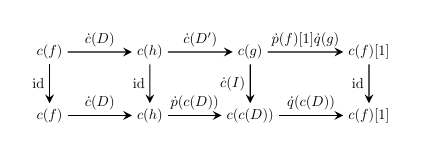
\begin{tikzpicture}[>=stealth,scale=0.52,every node/.style={transform shape}]
    \node (cf1) at (0,1.55) {$c(f)$};
    \node (ch1) at (2.45,1.55) {$c(h)$};
    \node (cg1) at (4.90,1.55) {$c(g)$};
    \node (cfs1) at (7.80,1.55) {$c(f)[1]$};
    \node (cf2) at (0,0) {$c(f)$};
    \node (ch2) at (2.45,0) {$c(h)$};
    \node (ccd) at (4.90,0) {$c(c(D))$};
    \node (cfs2) at (7.80,0) {$c(f)[1]$};
    \draw[->] (cf1) -- node[above] {$\dot c(D)$} (ch1);
    \draw[->] (ch1) -- node[above] {$\dot c(D')$} (cg1);
    \draw[->] (cg1) -- node[above] {$\dot p(f)[1]\dot q(g)$} (cfs1);
    \draw[->] (cf2) -- node[above] {$\dot c(D)$} (ch2);
    \draw[->] (ch2) -- node[above] {$\dot p(c(D))$} (ccd);
    \draw[->] (ccd) -- node[above] {$\dot q(c(D))$} (cfs2);
    \draw[->] (cf1) -- node[left] {$\mathrm{id}$} (cf2);
    \draw[->] (ch1) -- node[left] {$\mathrm{id}$} (ch2);
    \draw[->] (cg1) -- node[left] {$\dot c(I)$} (ccd);
    \draw[->] (cfs1) -- node[left] {$\mathrm{id}$} (cfs2);
  \end{tikzpicture}
\end{center}
\VerdierSemanticAnchor{ch1-3-3-5-proof-complete}
是三角的同构。

\VerdierSemanticAnchor{ch1-3-3-6}
\noindent\textbf{3.3.6.} 设
$F\colon \mathcal{J}\longrightarrow\operatorname{comp}(C)$ 为函子。以
$\mathcal{F}\ell_n(\mathcal{J})$ 表示 $\mathcal{J}$ 中由 $n$ 个可复合态射组成的
序列所构成的范畴：$\mathcal{F}\ell_n(\mathcal{J})$ 的对象是 $\mathcal{J}$ 中的图式

\VerdierSemanticAnchor{ch1-3-3-6-object-diagram}
\[
  i_1\xrightarrow{f_1}i_2\xrightarrow{f_2}i_3
  \longrightarrow\cdots\xrightarrow{f_n}i_{n+1}.
\]
\VerdierSemanticAnchor{ch1-3-3-6-morphism}
设 $(i_p,f_p)$ 和 $(j_p,g_p)$ 是 $\mathcal{J}$ 中两个由 $n$ 个可复合态射组成的
序列。$\mathcal{F}\ell_n(\mathcal{J})$ 中从 $(i_p,f_p)$ 到 $(j_p,g_p)$ 的一个
态射是交换图式

\VerdierSemanticAnchor{ch1-3-3-6-morphism-diagram}
\begin{center}
  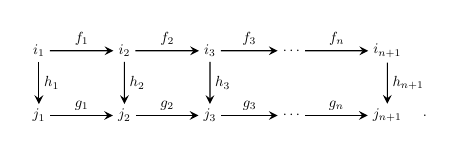
\begin{tikzpicture}[>=stealth,scale=0.53,every node/.style={transform shape}]
    \node (i1) at (0,1.55) {$i_1$};
    \node (i2) at (2.05,1.55) {$i_2$};
    \node (i3) at (4.10,1.55) {$i_3$};
    \node (idots) at (6.05,1.55) {$\cdots$};
    \node (in) at (8.35,1.55) {$i_{n+1}$};
    \node (j1) at (0,0) {$j_1$};
    \node (j2) at (2.05,0) {$j_2$};
    \node (j3) at (4.10,0) {$j_3$};
    \node (jdots) at (6.05,0) {$\cdots$};
    \node (jn) at (8.35,0) {$j_{n+1}$};
    \draw[->] (i1) -- node[above] {$f_1$} (i2);
    \draw[->] (i2) -- node[above] {$f_2$} (i3);
    \draw[->] (i3) -- node[above] {$f_3$} (idots);
    \draw[->] (idots) -- node[above] {$f_n$} (in);
    \draw[->] (j1) -- node[above] {$g_1$} (j2);
    \draw[->] (j2) -- node[above] {$g_2$} (j3);
    \draw[->] (j3) -- node[above] {$g_3$} (jdots);
    \draw[->] (jdots) -- node[above] {$g_n$} (jn);
    \draw[->] (i1) -- node[right] {$h_1$} (j1);
    \draw[->] (i2) -- node[right] {$h_2$} (j2);
    \draw[->] (i3) -- node[right] {$h_3$} (j3);
    \draw[->] (in) -- node[right] {$h_{n+1}$} (jn);
    \node at (9.25,0) {$.$};
  \end{tikzpicture}
\end{center}
\VerdierSemanticAnchor{ch1-3-3-6-composition}
态射的复合以显然的方式定义。以 $\mathrm{Fl}_n(\mathcal{J})$ 表示
$\mathcal{F}\ell_n(\mathcal{J})$ 的对象集。

\VerdierSemanticAnchor{ch1-3-3-6-cone-functor}
设 $i\xrightarrow{f}j$ 是 $\mathcal{F}\ell_1(\mathcal{J})$ 的对象。应用函子 $F$
得到 $\operatorname{comp}(C)$ 中的态射
\[
  F(i)\xrightarrow{F(f)}F(j),
\]
它可视为 $\operatorname{Tr}_1(C)$ 的对象；于是应用映射锥函子得到函子
$S\colon\mathcal{F}\ell_1(\mathcal{J})\longrightarrow\mathrm{K}(C)$：

\VerdierSemanticAnchor{ch1-3-3-6-1}
\begin{equation}
  S(f)=S\bigl(i\xrightarrow{f}j\bigr)
  =c\bigl(F(i)\xrightarrow{F(f)}F(j)\bigr).
  \tag{3.3.6.1}
\end{equation}
\endgroup
